%; whizzy document
% latex beamer presentation.
% platex, latex-beamer $B$G%3%s%Q%$%k$9$k$3$H$rA[Dj!%(B 

% $B<B9T=gHV(B
% sudo  ~/bin/usb-macbook-ir.c &
% real presentation (shell-command (concat "DISPLAY=:0.1 xpdf -fullscreen " (replace-regexp-in-string "tex$" "pdf"(buffer-file-name)) "&"))
% DISPLAY=:0.1 xpdf -fullscreen 

\documentclass[cjk,dvipdfm]{beamer}
\usetheme{Warsaw}
%  preview (shell-command (concat "xpdf " (replace-regexp-in-string "tex$" "pdf"(buffer-file-name)) "&"))
%  presentation (shell-command (concat "xpdf -fullscreen " (replace-regexp-in-string "tex$" "pdf"(buffer-file-name)) "&"))

%http://www.naney.org/diki/dk/hyperref.html
%$BF|K\8l(BEUC$B7O4D6-$N;~(B
\AtBeginDvi{\special{pdf:tounicode EUC-UCS2}}
%$B%7%U%H(BJIS$B7O4D6-$N;~(B
%\AtBeginDvi{\special{pdf:tounicode 90ms-RKSJ-UCS2}}

\title{Wonderful World of Mactel Debian }
\subtitle{TLUG}
\author{Junichi Uekawa dancer@debian.org}
\date{2006$BG/(B7$B7n(B29$BF|(B}

\logo{
\includegraphics[width=8cm]{image200607/openlogo-light.eps}}


% $B;0BrLdBjMQ(B
\newcounter{santakucounter}
\newcommand{\santaku}[5]{%
\addtocounter{santakucounter}{1}
\frame{\frametitle{$BLdBj(B\arabic{santakucounter}. #1}
%$BLdBj(B\arabic{santakucounter}. #1
\begin{minipage}[t]{0.7\hsize}
 \begin{itemize}
 \item $B""(B A #2\\
 \item $B""(B B #3\\
 \item $B""(B C #4\\
 \end{itemize}
\end{minipage}
}
\frame{\frametitle{$BLdBj(B\arabic{santakucounter}. #1}
%$BLdBj(B\arabic{santakucounter}. #1
\begin{minipage}[t]{0.7\hsize}
\begin{itemize}
\item $B""(B A #2\\
\item $B""(B B #3\\
\item $B""(B C #4\\
\end{itemize}
\end{minipage}
\begin{minipage}[t]{0.2\hsize}
$BEz$($O(B:


\vspace{1cm}

{\huge \hspace{1cm}#5}
\end{minipage}}
}


\begin{document}
\frame{\titlepage{}}



\section{Intro}

\begin{frame}
\frametitle{Who am I?}
\begin{itemize}[<+->]
 \item Junichi Uekawa $B>e@n(B $B=c0l(B
 \item Debian Developer
 \item Bought MacBook at end of June 2006
\end{itemize}
\end{frame}

\section{Why Debian on Macbook}

\begin{frame}
\frametitle{What's new in Debian on MacBook}
\begin{center}
\begin{minipage}{0.8\hsize}
  \begin{itemize}
   \item New architecture\\
	Boots with EFI\\
	Want to play with machine with weird architecture

   \item Everything is connected via USB, including built-in keyboard,
	mouse, iSight, IR-remote.
   \item Intel Core Duo: dual-core CPU
 \end{itemize}
\end{minipage}
\end{center}
\end{frame}

\begin{frame}
\frametitle{EFI: a Good News}

\begin{tabular}[t]{|p{8em}|p{8em}|p{8em}|}
\hline
 & BIOS & EFI \\
\hline
Partition & MBR: 4 (basic) & GPT: 128 \\
\hline
Filesystem & Mystery & Reads FAT \\
\hline
Execution format & What? & PE32+ \\
\hline
\end{tabular}
\end{frame}


\begin{frame}
\frametitle{EFI: command-line}

Allows use of MS-DOS-like command-line\\
You can enter commands even before boot-loader starts!

EFI$>$ fs0:\\
EFI fs0:$>$ cd EFI\\
EFI fs0:$\backslash{}$EFI$>$ cd dancer\\
EFI fs0:$\backslash{}$EFI$\backslash{}$dancer$>$ cd refit\\
EFI fs0:$\backslash{}$EFI$\backslash{}$dancer$\backslash{}$refit$>$ dir\\
refit.efi\\
 EFI fs0:$\backslash{}$EFI$\backslash{}$debian$\backslash{}$refit$>$ refit

\end{frame}

\section{Debian on Macbook}

\begin{frame}
 \frametitle{dual-booting Mac OS X and Debian}
 \begin{minipage}{0.5\hsize}
  \begin{itemize}
   \item Buy MacBook
   \item Process partition from Mac OS X
   \item Install rEFIt 
   \item Install Debian
   \item Configuration
  \end{itemize}
 \end{minipage}
\end{frame}

\subsection{Buy MacBook} 

\begin{frame}
 \frametitle{Buy MacBook}
 \begin{minipage}{0.5\hsize}
  \begin{itemize}
   \item Click!
  \end{itemize}
 \end{minipage}
\end{frame}

\subsection{Process partition from Mac OS X}

\begin{frame}
 \frametitle{Process partition from Mac OS X}
\begin{itemize}
 \item Online resize possible with recent Mac OS X\\
       \texttt{Mac OS X$\sharp$  sudo diskutil resizevolume disk0s2 20G}
\end{itemize}
\end{frame}

\subsection{Install rEFIt}

\begin{frame}
 \frametitle{Install rEFIt}
 \begin{itemize}
  \item run bless on Mac OS X, make rEFIt at boot
  \item When downloading binary from \url{http://refit.sourceforge.net/}
  \begin{itemize}
   \item Extract files to \texttt{/efi}, or somewhere
   \item Run \texttt{./enable.sh} (It will run \texttt{bless} for you)
  \end{itemize} 
  \item When using Debian refit package
  \begin{itemize}
   \item copy \texttt{/usr/lib/refit/} to Mac OS X partition
   \item \texttt{sudo bless --folder [full path to directory with
	 refit.efi] --file [full path to refit.efi]}
  \end{itemize}
 \item rEFIt screen will show after a reboot
 \end{itemize}
\end{frame}

\begin{frame}
\frametitle{Boot sequence}
\begin{minipage}[t]{0.4\hsize}
% dot -Tps -o bootchain.ps bootchain.dot
\includegraphics[height=1\hsize]{image200607/bootchain.ps}
\end{minipage}
\begin{minipage}[t]{0.58\hsize}
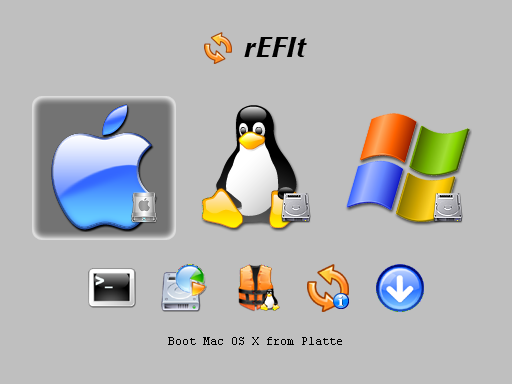
\includegraphics[width=1\hsize]{image200607/screen1.png}
\end{minipage}
\end{frame}

\subsection{Install Debian}

\begin{frame}
 \frametitle{Install Debian}
\begin{itemize}
 \item etch after July 2006 will probably work\\
       Install partition must be partition 3 or 4.
 \item Boot loader is lilo, but it won't work
 \item parted will create GPT table, but destroy MBR.\\
       move to command-console with Alt-F2\\
       synchronise with gptsync command\\
       return with Alt-F1
 \item Install lilo to partition
 \item Linux is now selectable from rEFIt after reboot
\end{itemize}
\end{frame}

\begin{frame}
\frametitle{MBR vs GPT}
Shows up differently even on same disk\\
\begin{minipage}[t]{0.68\hsize} 
MBR

{\scriptsize
 Disk /dev/sda: 80.0 GB, 80026361856 bytes\\
255 heads, 63 sectors/track, 9729 cylinders\\
Units = cylinders of 16065 * 512 = 8225280 bytes\\

   Device Boot      Start         End      Blocks   Id  System\\
/dev/sda1               1          26      204819+  ee  EFI GPT\\
/dev/sda2              26        2637    20971520   af  Unknown\\
/dev/sda3   *        2637        2758      976563   ef  EFI (FAT-12/16/32)\\
/dev/sda4            2758        5190    19531250+  ef  EFI (FAT-12/16/32)\\
}
\end{minipage}
\begin{minipage}[t]{0.30\hsize}
GPT\\

{\small
 major minor  $\sharp{}$blocks  name\\

   8     0   78150744 sda\\
   8     1     204800 sda1\\
   8     2   20971520 sda2\\
   8     3     976563 sda3\\
   8     4   19531250 sda4\\
   8     5    2929688 sda5\\
}
\end{minipage}
\end{frame}

\subsection{Configuration}

\begin{frame}
 \frametitle{X configuration}
\begin{itemize}
 \item i810
 \item use 915resolution$B!!(Bto set to 1280x800
 \item \texttt{xkbset m} will help with lack of right/middle mouse buttons
\end{itemize}
\end{frame}

\begin{frame}
 \frametitle{kernel configuration}
\begin{itemize}
 \item Older kernels before 2.6.17 seems to panic 4/5 times.
 \item rtc.ko seems to be broken, use rtc-dev.ko
 \item sound:\texttt{snd\_hda\_intel}
 \item NW: sky2\\
       wifi: madwifi
 \item CPU frequency can be controlled with \texttt{cpufreq\_centrino};
       \texttt{apt-get install cpufreqd}
\end{itemize}
\end{frame}

\begin{frame}
 \frametitle{madwifi}
 \begin{itemize}
  \item \texttt{sudo apt-get install madwifi-source madwifi-tools madwifi-doc}
  \item \texttt{sudo m-a prepare}
  \item \texttt{sudo m-a a-i madwifi}
  \item \texttt{sudo modprobe ath\_pci}
  \item<2-> sometimes seems to hang at boot; stability is not too good.
 \end{itemize}
\end{frame}

\begin{frame}
 \frametitle{linux-uvc}
 \begin{itemize}
  \item \texttt{sudo apt-get install linux-uvc-source linux-uvc-tools}
  \item \texttt{sudo m-a prepare}
  \item \texttt{sudo m-a a-i linux-uvc}
  \item \texttt{sudo mount /dev/sda2 /mnt/mac}
  \item \texttt{sudo macbook-isight-firmware-loader \\
       /mnt/mac/System/Library/Extensions/IOUSBFamily.kext/\\Contents/PlugIns/AppleUSBVideoSupport.kext/\\Contents/MacOS/AppleUSBVideoSupport}
  \item \texttt{sudo modprobe uvcvideo}
  \item \texttt{sudo apt-get install ekiga libpt-plugins-v4l2}
 \end{itemize}
\end{frame}

\begin{frame}
 \frametitle{linux-uvc}
 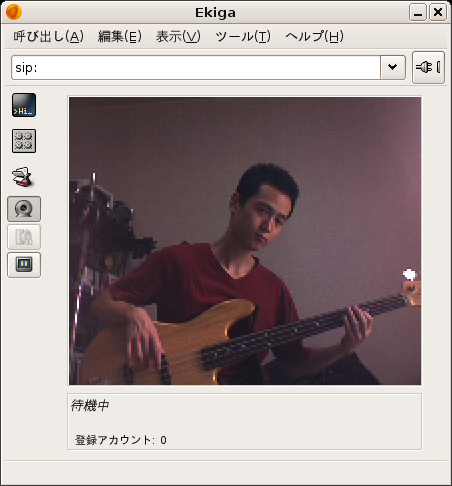
\includegraphics[width=0.8\vsize]{image200607/ekiga.png}
\end{frame}

\section{Other goals}

\subsection{What I hacked}

\begin{frame}
 \frametitle{Patches I made for this presentation}

Using Debian enough for preparing for presentations.

 \begin{itemize}[<+->]
  \item 377198: module-assistant: kernel modules cannot be built for 2.6.18-rc1
  \item 247602: xpdf-reader: fullscreen with metacity and other NETWM
	window managers
  \item IR receiver hack: do presentation with IR remote.
  \item Debian refit package
  \item linux-uvc package
 \end{itemize}
\end{frame}

\subsection{IR remote}

\begin{frame}
 \frametitle{USB device}

\begin{minipage}[t]{0.4\hsize}
  \begin{itemize}
  \item<1-> IR remote
  \item<1-> USB HID device
  \item<2-> libusb and libXtst\\
       3-minute hacking
  \item<3-> There is already a kernel driver, you could do all this with
       xmodmap.
 \end{itemize}
\end{minipage}
\begin{minipage}[t]{0.5\hsize}
 \onslide<2->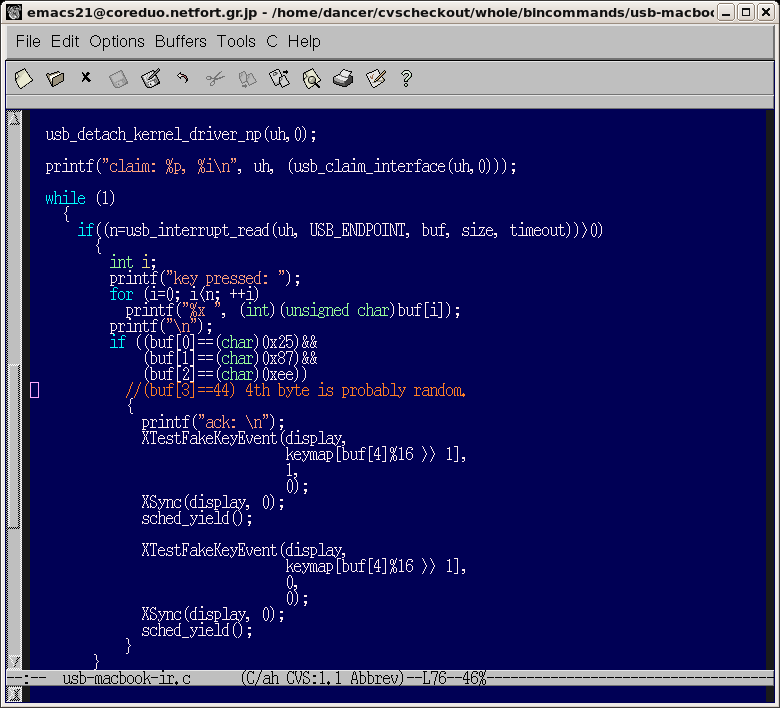
\includegraphics[width=2\hsize]{image200607/usbir.png}
\end{minipage}
\end{frame}



\begin{frame}
\frametitle{What next?}
Devices that I haven't touched yet
\begin{itemize}
 \item suspend/sleep
 \item CD-R writing
 \item backlight control
 \item bluetooth
 \item other yet unknown features ..
\end{itemize}
\end{frame}

\end{document}
